\documentclass[11pt]{article}
\usepackage{ucs} %sami letters\renewcommand
\usepackage[utf8x]{inputenc}
\usepackage[T1]{fontenc}
\usepackage{eacl2009}
\usepackage{times}
\usepackage{url}
\usepackage{latexsym}
\usepackage{linguex}

\setlength{\intextsep}{1ex}

\usepackage{graphics}


\begin{document}

\title{A constraint grammar for Faroese}
\author{Trond Trosterud \\ 
University of Tromsø}

\date{}

\maketitle{}

\begin{abstract}
The present paper presents ongoing work on a finite-state transducer, a Constraint Grammar disambiguator and dependency grammar for Faroese. In Faroese, the classical Germanic system of case, person and number inflection is upheld, but with somewhat more homonymy than in the closely related Icelandic. Rather than conflating homonym categories, the present morphological transducer gives a fully specified analysis of all morphological distinctions.
\end{abstract}

\section{Introduction} 

... two words about the parser ...

The transducer is based upon the lemma list of \emph{Føroysk órðabók} (\cite{Poulsen98})\footnote{Thanks to the authors for making lemmalist and inflection codes electronically accessible, Without it this project would of course not have been realisable.}, and upon the grammatical description found in \cite{Thr04}. 

The Faroese parser uses the computational infrastructure from the Sámi parser project (\textit{giellatekno.uit.no}). It has the same file setup, similar makefiles, etc. There are also benefits in the opposite relation: The Sámi morphophonology testsuite was taken from work on the Faroese \textit{twolc} file. 

The Faroese morphological analyser/generator \textit{Ffst} is a finite-state transducer. It is compiled with Xerox transducer compilers: \textit{twolc} for Morphophonology, and \textit{lexc} for lexicon and morphology (cf. \cite{Beesley03} and \url{http://www.fsmbook.com/}). The disambiguator \textit{Fdis} and dependency grammar \textit{Fdep} are written within the Constraint Grammar framework (see e.g. \cite{Karlsson90}, \cite{Karlsson95}), and uses the 3rd generation compiler \textit{vislcg3} (\cite{Bick00}, \url{http://beta.visl.sdu.dk/cg3.html}).

Sections 2, 3 and 4 present the grammatical analyser Ffst, the disambiguator Fdis and the dependency grammar Fdep, respectively. Section 5 gives an evaluation of the current stand of the parser, and the final section contains future perspectives and a conclusion.

\section{The grammatical analyser}




\subsection{Lexicon}

The analyser uses the same inflectional codes as  \cite{Poulsen98}.  New words annotated with the same codes may thus be added directly to the Ffst. The analyser has a dynamic compounding component, genitive singular nouns have the basic noun lexicon as one of their continuation lexica, thereby creating a loop allowing any compound with genitive singular first part. This gives rise to a circular automaton, for generation this component must thus be switched off.

Ffst also contains a name guesser. The guesser detects words with capital first letter and non-Faroese phonotax. The candidate words must contain at least one vowel. The final letter cannot be a Faroese suffixal sound (\textit{a, i, u, n, m, r, s, t} (to avoid explicit case endings). The putative name is then assigned Nom, Acc and Dat. If there is any other analysis available, the guessed form is automatically discarded. The guesser is very reliable: Of the 500 most common guesses all 500 were actually names. It is also (too) careful: Banning Faroese case suffixes from the guesser avoids analysig case-inflected forms as baseforms, but at the same time it prevents the parser from making many correct guesses. 


\subsection{Morphology}

The morphological part of \textit{Fdis} is built in several layers. For the nominal morphology, the first layer gives the part of speech and gender tags, and morphophonological flags, as shown in Figure \ref{bondi}, for the noun \textit{bóndi} “farmer”, where the nominative and accusative plural forms show Umlaut.

\begin{figure}[hp]
\begin{center}
\scalebox{0.55}[0.55]{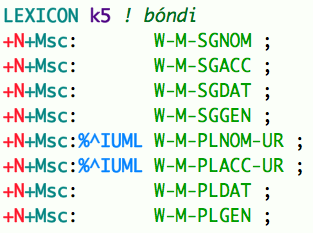
\includegraphics{img/bondi.png}}
\caption{Definiteness morphology}
\label{bondi}
\end{center}
\end{figure}

The dictionary contains xx nominal declension types, but including singular-only and plural-only declension patterns, and combined patterns (words declined for more than one pattern), the system totals 269 distinct first-layer continuation lexica for nouns, one of them being the $k5$ lexicon in Figure \ref{bondi}.

The second layer gives case and number morphology. Figure \ref{wmplnom} gives the continuation lexica for weak masculine plurals, i.e., also for \textit{bóndi} and the other $k5$ words. 
 
\begin{figure}[hp]
\begin{center}
\scalebox{0.40}[0.40]{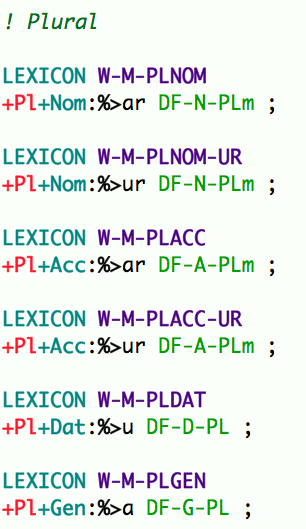
\includegraphics{img/wmplnom.png}}
\caption{Second layer - case and number}
\label{wmplnom}
\end{center}
\end{figure}

The third layer gives definiteness morphology. Due to the agglutinative nature of Faroese morphology, the lexica either only add the indefinite tag, or the definite tag and suffix. The exception is dative, which shows an \textit{n:m} alternation. Rather than writing a morphophonological rule deleting \textit{m} in front of \textit{num}, the alternation is written into the morphology file.

\begin{figure}[htp]
\begin{center}
\scalebox{0.3}[0.3]{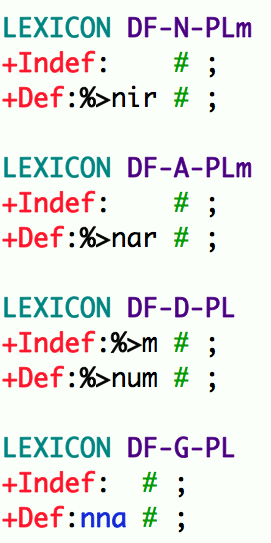
\includegraphics{img/dfnplm.png}}
\caption{Third layer - definiteness}
\label{dfnplm}
\end{center}
\end{figure}
 

Applying these lexica, we get, among others the accusative and dative plural definite forms shown in Figure \ref{lexcstring}.  

\begin{figure}[htp]
\begin{center}
\scalebox{0.320}[0.320]{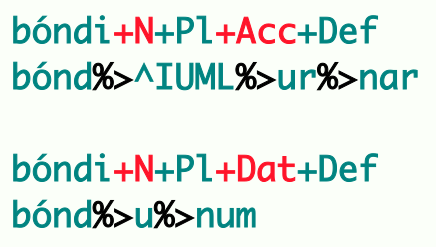
\includegraphics{img/bondi_lexc.png}}
\caption{The resulting upper and lower lexc strings}
\label{lexcstring}
\end{center}
\end{figure}

\subsection{Morphophonology}

The lower part of the string pairs from the morphological transducer are then fed to a separate automaton, the morphophonological component. This automaton contains rules for morphophonological alternations, and for non-segmental morphology. The relevant rule in this context is \textit{I-umlaut}, shown in figure \ref{twoliumlaut}. The rule works on strings containing any of the vowels in Vx, zero or more consonants, and the Umlaut trigger symbol \symbol{94}IUML, and changes all vowels in Vx into the corresponding vowels in Vy. In this case, it changes \textit{ó} into \textit{ø}.
 
\begin{figure}[htbp]
\begin{center}
\scalebox{0.35}[0.35]{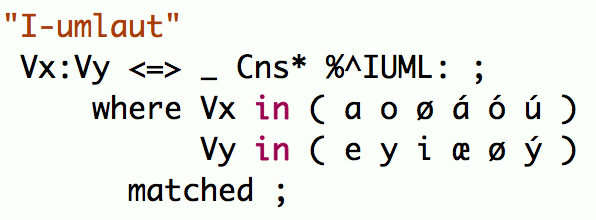
\includegraphics{img/twoliumlaut.png}}
\caption{The twolc i-umlaut rule}
\label{twoliumlaut}
\end{center}
\end{figure}

The morphological and morphophonological transducers are then composed, and the resulting transducers gives a pairing of the upper represenation of the former and the lower represntation of the latter, graphically presented in Figure \ref{automaton}, with the invisible, intermediate strings shown in shaded grey.

\begin{figure}[hp]
\begin{center}
\scalebox{0.43}[0.43]{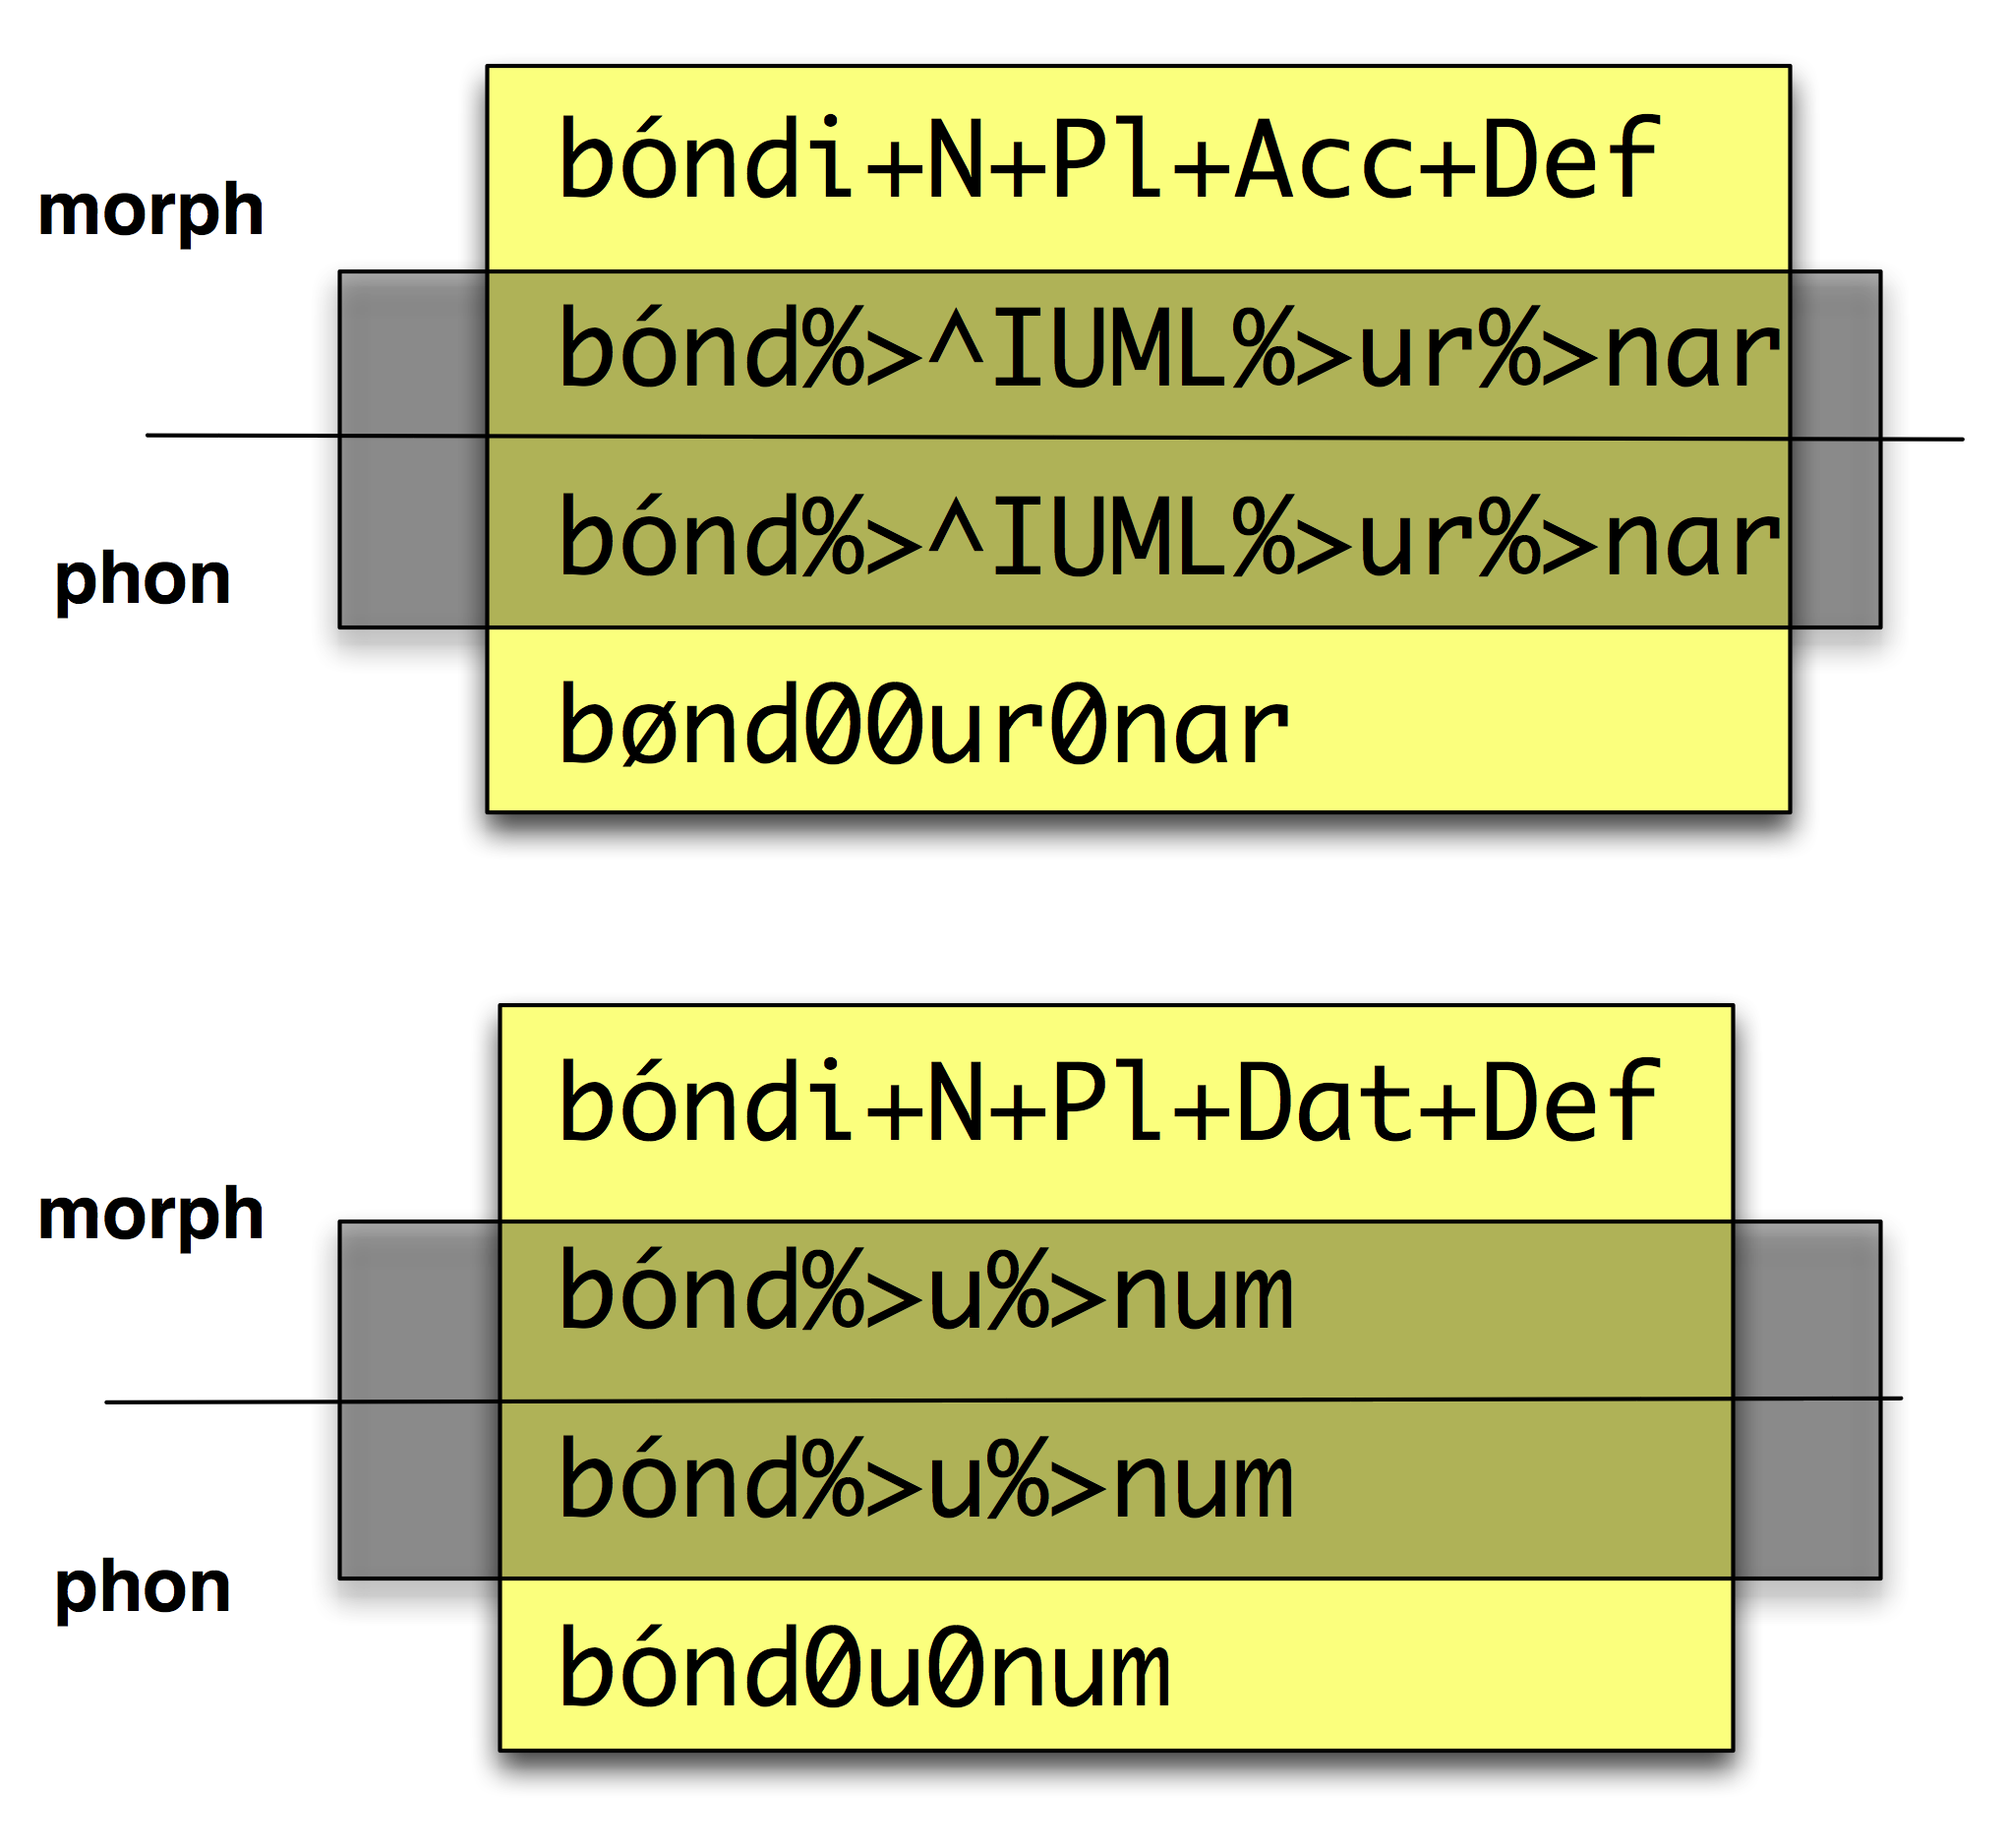
\includegraphics{img/automaton.png}}
\caption{The transducers}
\label{automaton}
\end{center}
\end{figure}

Applied to all grammatical words of the lexeme \textit{bóndi}, Ffst gives the paradigm shown in Figure \ref{bondiparadigm}.

\begin{figure}[hp]
\begin{center}
\scalebox{0.31}[0.31]{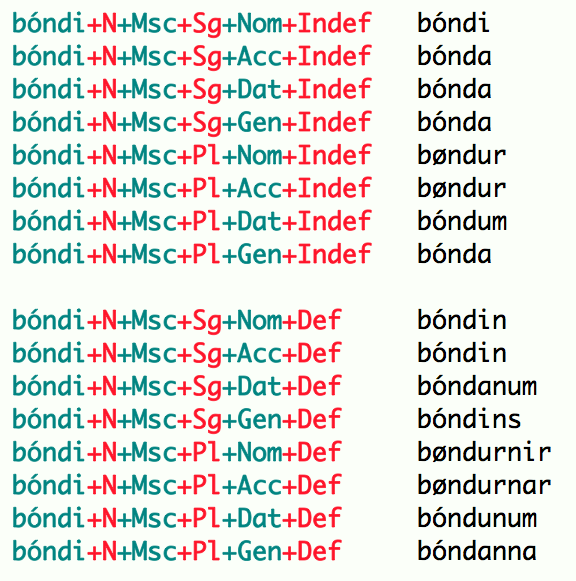
\includegraphics{img/bondiparadigm.png}} 
\caption{The resulting paradigm for bóndi}
\label{bondiparadigm}
\end{center}
\end{figure}

A list of the morphophonological rules is given in Figure \ref{twolrules} on page \pageref{twolrules}.

\begin{figure*}[htbp]
\begin{center}
\scalebox{0.4}[0.4]{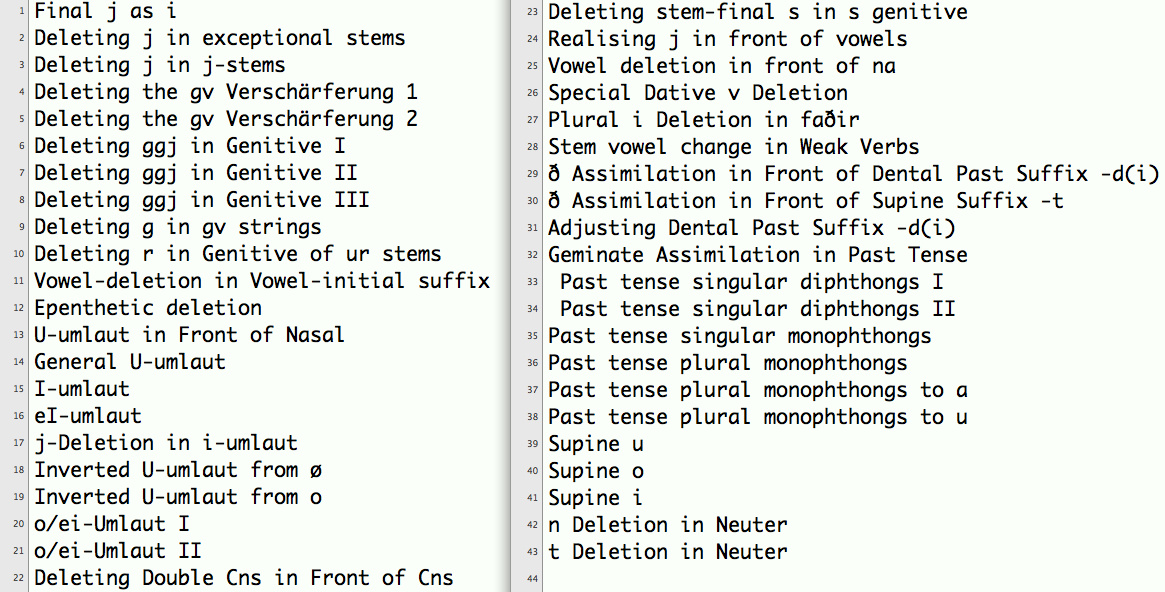
\includegraphics{img/twolrules.png}}
\caption{Twol rules}
\label{twolrules}
\end{center}
\end{figure*}



\subsection{Status quo for Ffst}


At present (May 2009), the Faroese morphological transducer recognises 93.5 \% of all wordform tokens and 62.8 \% of all wordform types in running text (the discrepancy indicates that Ffst handles common words better than rare ones). 

The results could still be better, but for certain subgenres (such as the Bible), Ffst gives better results (96.3 \% and 83.3 \%, respectively), results good enough to evaluate the subsequent CG component. Note that even for the known text, Ffst misses approximately 16 \% of the wordform types. The reason for this high number is that certain parts of the transducer are still under construction, especially parts of the irregular verbs, and of comparative and superlative forms of adjectives.

\begin{itemize}
\setlength{\itemsep}{-0.2cm}
\item The parser recognises 94.3 \% of the wordforms and 63.3  \% of the wordform types in running text
\item The discrepancy indicates that Ffst handles common words better than rare ones
\item{Certain common forms are missing (some strong verbs, irregular adjective forms, comparatives (partly))}
\item{Faroese names are missing (except the most central person names), but many are taken care of by the guesser}
\end{itemize}


The top 84 missing wordforms from an 2.7 m wd corpus are shown in Figure \ref{84miss} on page \pageref{84miss}. 

\begin{figure*}[htbp]
\begin{center}
\scalebox{0.5}[0.5]{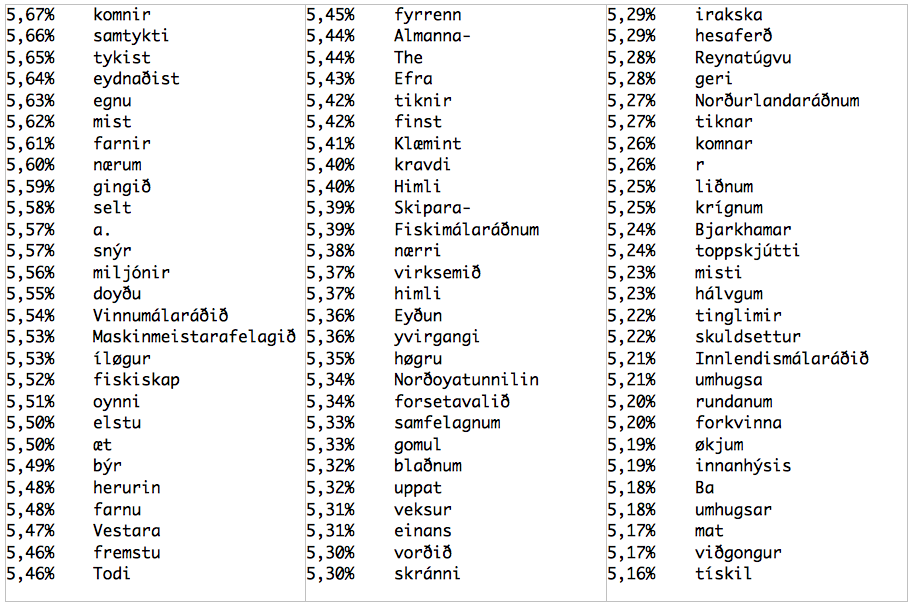
\includegraphics{img/missing.png}}
\caption{Top 84 missing wordforms, the percentages showing the percentage of the corpus left unanalysed with a list of missing wordforms up to and including the wordform in question}
\label{84miss}
\end{center}
\end{figure*}


The 43093 missing wordforms represent 5.67\% of the 2.7 mill corpus. In order to reduce the number of missing wordforms in running text by 50\%, the top 2117 wordforms of the missing list would have to be added to the analyser. Important areas for lexicon improvement include the following:

\begin{itemize}
\setlength{\itemsep}{-0.2cm}
\item Adjectival inflection of participles, irregular adjectival forms
\item Some irregular strong verbs and verb forms
\item Faroese names (other than person names)
\item Compounded function words
\item Words missing from FÓ
\item Plain errors
\end{itemize}




\section{The Faroese disambiguator}

The disambiguator (Fdis) consists of 120 rules for morphological disambiguation,  49 mapping rules, and 46 rules for disambiguation of grammatical functions. This is a small, but relatively efficient rule set, compared to the disambiguators for some other languages in Table \ref{rulecount}\footnote{The Sámi parsers are developed at the University of Tromsø (UiT), the Greenlandic parser is joint work between Oqaasileriffik and UiT, and the Bokmål parser is developed at Tesktlaboratoriet in Oslo}. For each language, the table gives number or rules, and the average numbers of readings before and after disambiguation, as applied on a compatible corpus (Genesis and the New Testament).

\begin{table}[htdp]
\caption{Rules and results for some CG parsers}
\begin{center}
\begin{tabular}{|l|c|c|c|}
\hline
Parser & Rules & Input & Output \\
\hline
North Sámi	  & 3537 & 2.42 & 1.08 \\
Norsk Bokmål  & 1964 & 2.13 & 1.17 \\
Lule Sámi	  &  832 & 2.18 & 1.21 \\
Faroese		  &  294 & 2.45 & 1.24 \\
Greenlandic	  &  518 & 2.69 & 1.42 \\
\hline
\end{tabular}
\end{center}
\label{rulecount}
\end{table}%

\subsection{Tag unification}

The efficiency of the Fdis ruleset illustrates the efficiency of an innovation in vislcg3, namely set unification for tags. With the set unification operator $\$\$$ it is possible to refer to a set, so that the tag that first satisfies the set must be the same as all subsequent matches of the same set. Cf. the rule \ref{selectnagd}, which refers to the set \ref{setnagd}.

\begin{flushleft}
\ex.\label{selectnagd} \small{SELECT \$\$NAGD IF (0 Det)(*1C \$\$NAGD BARRIER NOT-NP);}

\ex.\label{setnagd} \small{SET NAGD = Nom Acc Gen Dat ;}
\end{flushleft}


The disambiguator (Fdis) consists of 120 rules for morphological disambiguation, 49 mapping rules, and 46 rules for GF-disambiguation. The dependency grammar (Fdep) consists of 49 rules. With this rule set, Fdis works with an accuracy of 1.14 (an average of 1.14 analyses per word in running text), on an input where the wordforms on average had 3.01 analyses (the results were obtained on a corpus of 100000 words of newstext , previously not used for rule development, disregarding the unknown words, who had no cohorts to disambiguate).

Remarkable here is the low number of disambiguation rules. A standard CG grammar usually has several thousand rules. Partly, the low number of rules in Fdis reflects the intermediate status of the parser, and also its low accuracy (for a CG parser an accuracy of 1.14 is not a good result), but partly it illustrates the efficiency of an innovation in vislcg3, namely set unification for tags. With the set unification operator \$\$ it is possible to refer to a set, so that the tag that first satisfies the set must be the same as all subsequent matches of the same set. Cf. (\ref{NAGD}), where the case of the determiner is selected based upon any unambiguous case form within the same NP.

\ex.\label{NAGD} \small{SELECT \$\$NAGD IF (0 Det)(*1C \$\$NAGD BARRIER NOT-NP);}

The bulk of the rules aims at disambiguating case, number and gender within the NP. One clue as to determining the correct case is the choice of preposition, as it is for the human listener. Unfortunately, most Faroese prepositions subcategorise for more than one case. What case to choose if there is a tie is ultimately dependant upon the combination of verb and preposition. At the present stage, Fdis does not specify subcategorisation frames for verbs and verb + preposition combinations, this is an area for future improvement.

When disambiguating running text, certain high-frequent words need special attention, both because they get multiple interpretations in the morphological component, and for their key role in the sentence. A common strategy for such words is to write specific rules just for these words. For Fdis, only approximately 15 such words have received special treatment until now, among them the pronouns \textit{hon, vit} and the ambiguous function words \textit{at, ið, men}. Also this is an area for improvement.

The Faroese verbal paradigm shows much homonymy. Ffst follows the practice of the reference grammars, and specifies 3 persons in the singular (also when the conjugation in question shows homonymy), but only one plural form. Naturally, disambiguating of the verbal forms rests heavily upon the person of the subject. 

Mapping of grammatical functions is done on the basis of morphological cues and word order, and their disambiguation mainly on the basis of word order. The grammatical function tags are directional (the distinction @OBJ> / @<OBJ indicates whether the governing verb is to found to the right or to the left, respectively). This distinction is heavily utilised in the dependency grammar.

The dependency grammar quite reliably delimits NPs, and the governed constituents of P and V. Eventual errors here are due to errors in Fdis. The main obstacles for a good depencency analyses are coordination and relative clauses. Attaching appropriate constituents to the clause mother node is quite a reliable process as long as the rest of the analysis is correct. Unfortunately shortcomings in coordination and relative clause analysis, and especially the low coverage of the Ffst gives too many top nodes (2.3 alleged clausal heads per clause on average, compared to the correct 1 head/clause). Even with these shortcomings, the Fdep is already at this stage a good tool for research on basic dependency relations.

Unfortunately, most Faroese prepositions subcategorise for more than one case.  The choice of case is ultimately dependant upon the combination of verb (or sentence frame) and preposition.  Fdis selects Accusative for motion verbs and change of relationship PPs, otherwise it chooses Dative.

\subsection{High-frequent ambiguous words}

Certain high-frequent words need special attention, both because they get multiple interpretations in the morphological component, and for their key role in the sentence. A common strategy for such words is to write specific rules just for these words.  For Fdis, only approximately 15 such words have received special treatment until now, mainly pronouns (\textit{hon, vit, ..}) and subjunctions (\textit{at, ið, men, ...}).

\subsection{Verb homonymy}

The Faroese verbal paradigm shows much homonymy.  Ffst specifies 3 persons in the singular (also when the conjugation in question shows homonymy), but there is only one plural form, which, according to the Faroese grammatical tradition, is not disambiguated further.

\subsection{Grammatical functions}

The input to Fdis contains morphological information only. During Fdis analysis grammatical functions are mapped onto each reading on the basis of morphological cues, word order, and thereafter disambiguated on the basis of word order. The grammatical function tags are directional ( @OBJ> / @<OBJ, meaning “I am an object, and my governor is to my right / left”). This distinction is heavily utilised in the dependency grammar.

\section{The dependency grammar}

The dependency grammar (Fdep) consists of 49 rules. It quite reliably delimits NPs, and the governed constituents of P and V.  Eventual errors here are due to errors in Fdis.  The hard obstacles for a good depencency analyses are long-distance dependencies:  coordination and relative clauses, topicalisation.

\section{Evaluation}
\subsection{Precision and recall}

The parser was tested on a small corpus of 1033 words of unseen text from a new genre (Faroese education planning). The results are shown in Table \ref{prec}.


\begin{table}[htbp]
\caption{Precision, recall, accuracy and F-ms for a test corpus}
\begin{center}
\begin{tabular}{|l|r|r|r|r|}
\hline
Error type	& tp		& fp		& tn		& fn	\\
\hline
Morphology  &  2048  &  369  &  2501  &  101 \\ 
Syntax  &  1902  &  515  &  2357  &  245 \\  
Dependency &  724  &  316  &  0  &  0 \\
\hline
\hline
 & prec	 & rec.	& acc.	& F-ms. \\
\hline
Morphology    &  0.85  &  0.95  &  0.91  &  0.90 \\
Syntax    &  0.79  &  0.89  &  0.85  &  0.83 \\
Dependency  &  0.7  &  1  &  0.7  &  0.82 \\
\hline
\end{tabular}
\end{center}
\label{prec}
\end{table}%





Thus, Fdis is work in progress 

As an illustration of the Fdis output, consider Figure \ref{sent3} on page \pageref{sent3}. The two leftmost columns give the output from Ffst, with all possible readings. The third column gives the output from Fdis and Fdep, with ambiguity removed, and grammatical functions and dependency added.

\begin{figure*}[p]
\begin{center}
\scalebox{0.450}[0.450]{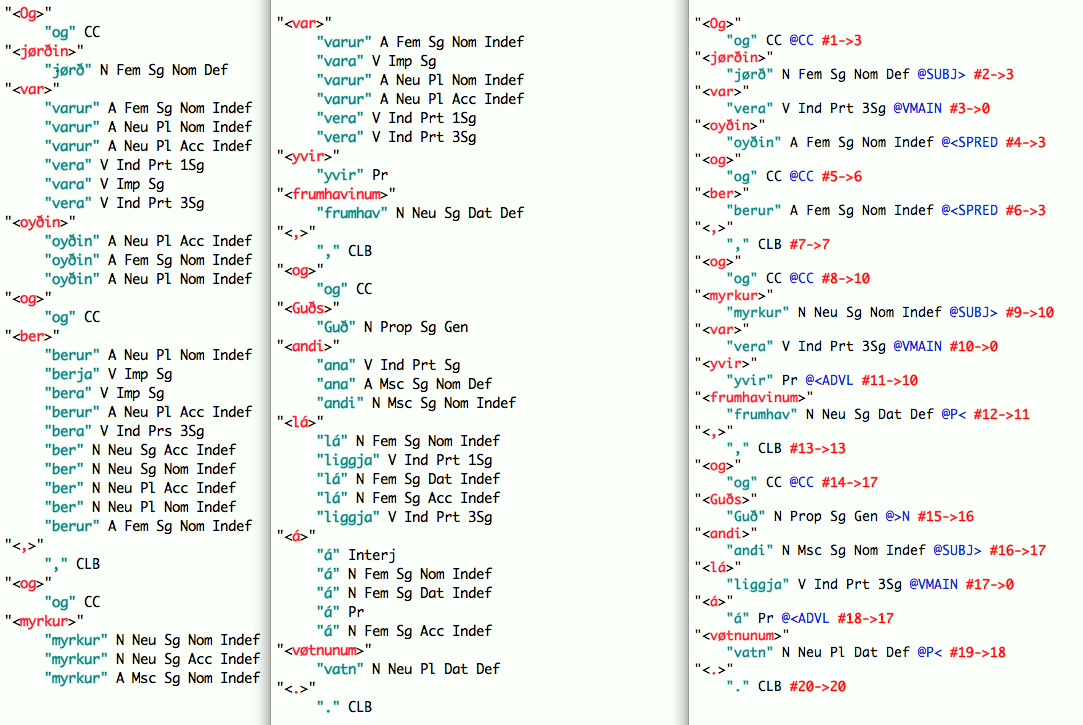
\includegraphics{img/frumhavinum.png}}
\caption{And the earth was waste and void; and darkness was upon the face of the deep: and the Spirit of God moved upon the face of the waters}
\label{sent3}
\end{center}
\end{figure*}
 
\subsection{Processing speed}

When it comes to processing speed, it seems that the bottleneck in the system is the disambiguator. Even though it is much smaller than most CG grammars, it performs clearly worse than all the other parts of the pipeline. The reason for this might be the extensive use of set unification.


\begin{table}[htdp]
\caption{Processing speed, measured on 100000 words of running text, on a 2,4 GHz laptop}
\begin{center}
\begin{tabular}{|l|l|r|}
\hline
Process & Program & Words/sec \\
\hline
Preprocessing & perl &10446 \\
Morphological lookup & fst & 42992 \\
Postprocessing & perl & 13017 \\
Disambiguation & vislcg3 & 2042 \\
Dependency & vislcg3 & 18814 \\
\hline
\end{tabular}
\end{center}
\label{time}
\end{table}%




\section{Conclusion}

The Faroese grammatical analyser presented here is still in the making. It still shows that with a modest number of CG rules, one may achive results good enough for several languaguage processing tasks. Future improvements of the analyser will concentrate upon key parts of the Ffst, upon disambiguation of complex syntactic patterns, and upon the dependency analysis of coordination and relative clauses.

\bibliography{/Users/trond/private/trunk/plan/art/bib/lgtech}
%\bibliography{$GTPRIV/plan/art/bib/lgtech}

\bibliographystyle{/Users/trond/private/trunk/plan/art/bib/acl2005}

\end{document}
